\documentclass{article}


% if you need to pass options to natbib, use, e.g.:
    \PassOptionsToPackage{numbers, compress}{natbib}
% before loading neurips_2024


% ready for submission
% \usepackage{neurips_2024}


% to compile a preprint version, e.g., for submission to arXiv, add add the
% [preprint] option:
    \usepackage[preprint]{neurips_2024}


% to compile a camera-ready version, add the [final] option, e.g.:
    % \usepackage[final]{neurips_2024}


% to avoid loading the natbib package, add option nonatbib:
  %  \usepackage[nonatbib]{neurips_2024}


\usepackage[utf8]{inputenc} % allow utf-8 input
\usepackage[T1]{fontenc}    % use 8-bit T1 fonts
\usepackage{hyperref}       % hyperlinks
\usepackage{url}            % simple URL typesetting
\usepackage{booktabs}       % professional-quality tables
\usepackage{amsfonts}       % blackboard math symbols
\usepackage{nicefrac}       % compact symbols for 1/2, etc.
\usepackage{microtype}      % microtypography
\usepackage{xcolor}         % colors
\usepackage{graphicx}       % for including graphics


\title{EE245 Project Proposal \\ \large A Study on Reinforcement Learning for Parking: Vision vs. Radar Sensing}


\author{
  Kunyi Yu\\
  Department of Computer Science and Engineering\\
  University of California, Riverside\\
  Riverside, CA 92521\\
  kyu135@ucr.edu
}

\begin{document}

\maketitle

% \begin{abstract}
%   The abstract \dots
% \end{abstract}

% 2 pages
% 1. Introduction and motivation – 20%
% 2. Task and datasets (example inputs & outputs, dataset statistics) – 20%
% 3. Literature review on existing work – 30%
% 4. Your novel idea: explain how it differs from existing work – 20%
% 5. Expected outcomes: what do you plan to achieve? – 10%

\section{Introduction and Motivation - 20\%}

Traffic accidents caused by human judgment errors remain a leading cause of fatalities worldwide. However, the rapid development of autonomous driving technologies holds promise for significantly reducing such incidents. In December 2024, the author visited the Bay Area and observed a growing presence of autonomous vehicles (AVs) on the road, either undergoing testing or already in commercial operation. Waymo, one of the industry pioneers, has been operating a fleet of AVs in San Francisco since August 2021. Unlike Waymo’s radar-based approach, Tesla’s Full Self-Driving (FSD) system relies primarily on vision-based sensing. Tesla’s commercial success demonstrates that a camera-only solution can be a viable alternative for autonomous driving.

Both radar and vision-based sensing solutions are widely researched and adopted in the industry, each with its own advantages and limitations. A 2024 news report \cite{news2024} highlighted an incident where Waymo’s AVs were excessively honking in a San Francisco parking lot, disturbing nearby residents multiple times at night. The issue was reportedly caused by interference from other vehicles, leading to a deadlock scenario—a common challenge in multi-agent systems. This also underscores the complexity and importance of autonomous parking as a research topic.

Motivated by these observations, this project aims to compare radar-based and vision-based sensing solutions in the context of autonomous vehicle parking, evaluating their performance in efficiency and safety under various reinforcement learning (RL) algorithms.

\section{Task and Experiment Setup - 20\%}

\textit{*Due to the nature of reinforcement learning, this section will not disscuss specific datasets.}

\texttt{highway-env} \cite{highway-env} is the simulation environment will be used. It is a widely used RL framework for autonomous driving research, offering various driving scenarios such as highway, merging, roundabout, and parking. The environment follows the OpenAI Gym Environment \texttt{gymnasium} \cite{towers2024gymnasium}, making it easy to integrate and customize. A parking scenario example is shown in figure below.

\begin{figure}[h!]
    \centering
    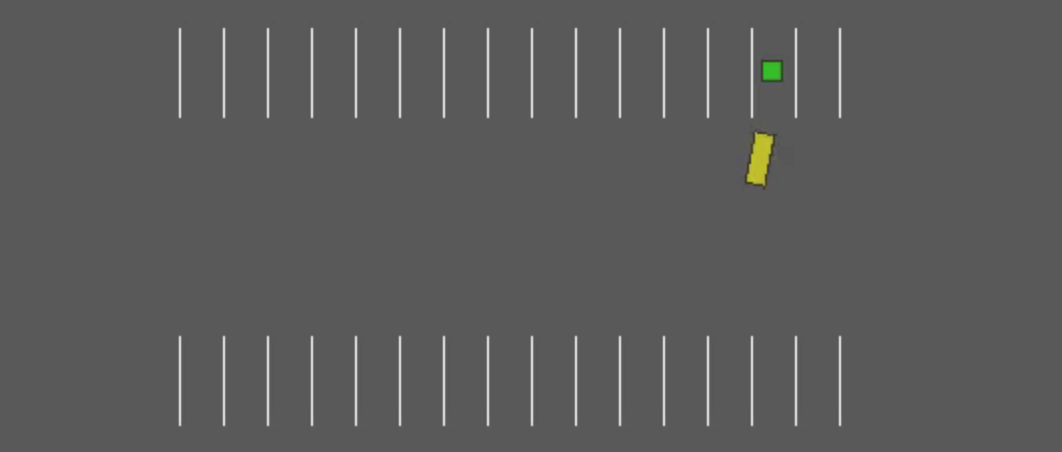
\includegraphics[width=0.4\textwidth]{./pics/parking.png}
    \caption{Parking scenario in the \texttt{highway-env} environment.}
\end{figure}

The goal is to train RL agents to park in simulated parking lots using different sensing modalities (vision vs. radar), and compare their performance. The task is structured into four milestones:

\begin{itemize}
    \item \textbf{Milestone 1 (Week 7)} – [1] Set up the \texttt{highway-env} environment with varying difficulty levels (empty, normal, almost-full); [2] Configure agent parameters, observation modalities, reward functions, and action spaces.
    \item \textbf{Milestone 2 (Week 8)} – [1] Train agents using different RL algorithms (e.g., DQN, PPO, A3C) in empty parking lots; [2] Evaluate performance based on efficiency (time to park) and safety (number of collisions).
    \item \textbf{Milestone 3 (Week 9)} – [1] Refine hyperparameters based on previous results; [2] Train and evaluate agents in normal and almost-full parking scenarios.
    \item \textbf{Milestone 4 (Week 10/11)} – [1] Compare the performance of vision-based and radar-based agents; [2] Summarize findings in the final report and presentation.
\end{itemize}

At the current stage, the author plans to use RGB/radar observation spaces, a continuous action space, and a sparse reward function penalizing collisions and parking time. Notably, continuous action spaces are incompatible with certain RL algorithms (e.g., DQN), and sparse rewards may pose challenges for training, requiring careful consideration. The implementation details still need to be discussed and modified in the future.

\section{Literature Review - 30\%}

This section will cover two parts: (1) The application of RL algorithms in autonomous parking; (2)Sensing modalities (vision-based or radar/lidar-based) in autonomous parking.

There are several papers study the autonomous parking problem directly in the \texttt{highway-env} environment. \citet{kapoor2020model} introduces a model-based RL approach that integrates neural dynamics prediction with STL-guided model predictive control, applied to robotics and autonomous driving. In the parking scenario, the algorithm can converge within 500k epochs but with a relatively high fluctuation in reward. \citet{moreira2021deep} proposes a deep reinforcement learning method with SAC, DDPG, and TD3 algorithms to teach a wheeled vehicle to park in confined spaces. However, the method needs to predefined the parking path manually. \citet{lazzaroni2023automated} presents a DRL-based agent trained in different environments (a Unity-based, highway-env, and CARLA) for low-speed parking maneuvers, achieving a 97\% success rate. The paper also uses Stable-Baselines3 \cite{stable-baselines3} toolkits for training the agents, which provides a set of reliable RL algorithm implementations. There also exist some YouTube videos \citep{youtube2019,youtube2022} visulizing the training process of reverse parking and parallel parking. A survey paper \cite{elallid2022comprehensive} provides a comprehensive overview of RL applications in autonomous driving, not limited to only parking scenarios.

\citet{yurtsever2020survey} provides a comprehensive survey on common practices and emerging trends. In the paper, there are serveral sensoring technologies are discussed, including vision-based sensors (monocular cameras, omnidirectional cameras, and event cameras), radar, and LiDAR (Point clouds). Firstly, \underline{vision-based sensors} have advantages in color sensing, passive sensing, and low cost due to established technology. However, their illumination sensitivity and difficulty in depth perception are significant drawbacks. \underline{Radar} sensors, on the other hand, have better long range detection, robustness to bad weather, and also low cost. However, they have lower resolution and their field of view is limited. Lastly, \underline{LiDAR} have pros in high accuracy, accuracy in depth perception, and robustness to illumination changes. However, they are expensive, heavy, and require large-scale data processing. If combing these sensors, the advantages of each sensor can be utilized.

\section{Novel Idea - 20\%}
In many research, sensoring modalities are not considered as a variable or usually over idealized. However, the author believes if reinforcement learning is used in the real world autonomous driving scenarios, a good sensing modality is crucial for people's safety the the public acceptance of AVs.

The noval idea of this project will be: (1) to compare the performance of vision-based and radar-based sensing solutions in the context of autonomous parking; (2) to evaluate the performance of different RL algorithms in the same environment with different sensing modalities.

The results of this project will provide insights into the pros and cons of each sensing modality, helping researchers and practitioners make informed decisions when designing AVs systems in real-world applications.

\section{Expected Outcomes - 10\%}

The expected outcomes of this project include:
\begin{itemize}
    \item final report and presentation slides
    \item a GitHub repository containing code and experiment results
\end{itemize}

\section*{Acknowledgements}
The author would like to thank Professor Jiachen Li and TAs for their patient guidance and help.



\bibliographystyle{unsrtnat}
\bibliography{refs}

\end{document}